\documentclass[10pt, a4paper]{article}

% Packages:
\usepackage[
    ignoreheadfoot, % set margins without considering header and footer
    top=2 cm, % seperation between body and page edge from the top
    bottom=2 cm, % seperation between body and page edge from the bottom
    left=2 cm, % seperation between body and page edge from the left
    right=2 cm, % seperation between body and page edge from the right
    footskip=1.0 cm, % seperation between body and footer
    % showframe % for debugging 
]{geometry} % for adjusting page geometry
\usepackage{graphicx} % for including images
\usepackage{titlesec} % for customizing section titles
\usepackage{tabularx} % for making tables with fixed width columns
\usepackage{array} % tabularx requires this
\usepackage[dvipsnames]{xcolor} % for coloring text
\definecolor{primaryColor}{RGB}{0, 79, 144} % define primary color
\usepackage{enumitem} % for customizing lists
\usepackage{fontawesome5} % for using icons
\usepackage{amsmath} % for math
\usepackage[
    pdftitle={Antoine's CV},
    pdfauthor={Antoine},
    pdfcreator={LaTeX with RenderCV},
    colorlinks=true,
    urlcolor=primaryColor
]{hyperref} % for links, metadata and bookmarks
\usepackage[pscoord]{eso-pic} % for floating text on the page
\usepackage{calc} % for calculating lengths
\usepackage{bookmark} % for bookmarks
\usepackage{lastpage} % for getting the total number of pages
\usepackage{changepage} % for one column entries (adjustwidth environment)
\usepackage{paracol} % for two and three column entries
\usepackage{ifthen} % for conditional statements
\usepackage{needspace} % for avoiding page brake right after the section title
\usepackage{tikz} % for creating graphics and diagrams
\usepackage{iftex} % check if engine is pdflatex, xetex or luatex

% Ensure that generate pdf is machine readable/ATS parsable:
\ifPDFTeX
    \input{glyphtounicode}
    \pdfgentounicode=1
    \usepackage[utf8]{inputenc}
    \usepackage{lmodern}
\fi

% Some settings:
\AtBeginEnvironment{adjustwidth}{\partopsep0pt} % remove space before adjustwidth environment
\pagestyle{empty} % no header or footer
\setcounter{secnumdepth}{0} % no section numbering
\setlength{\parindent}{0pt} % no indentation
\setlength{\topskip}{0pt} % no top skip
\setlength{\columnsep}{0cm} % set column seperation
\makeatletter

\titleformat{\section}{\needspace{4\baselineskip}\bfseries\large}{}{0pt}{}[\vspace{1pt}\titlerule]

% spacing around section titles
\titlespacing*{\section}
  {0pt}                              % left margin
  {3.0ex plus .5ex minus .2ex}       % before-title (rubber)
  {3.0ex plus .2ex minus .2ex}       % after-title  (rubber)

% paragraph skip
\setlength{\parskip}{1em plus 0.1em minus 0.1em}

% itemize/list spacing
\usepackage{enumitem}
\setlist[itemize]{
  topsep=0.2em plus 0.1em minus 0.1em,
  partopsep=0pt,
  parsep=0.1em plus 0.05em minus 0.05em,
  itemsep=0.1em plus 0.1em minus 0.05em,
  leftmargin=0.4cm
}

\renewcommand\labelitemi{$\circ$} % custom bullet points
\newenvironment{highlights}{
    \begin{itemize}[
        topsep=0.10 cm,
        parsep=0.10 cm,
        partopsep=0pt,
        itemsep=0pt,
        leftmargin=0.4 cm + 10pt
    ]
}{
    \end{itemize}
} % new environment for highlights

\newenvironment{highlightsforbulletentries}{
    \begin{itemize}[
        topsep=0.10 cm,
        parsep=0.10 cm,
        partopsep=0pt,
        itemsep=0pt,
        leftmargin=10pt
    ]
}{
    \end{itemize}
} % new environment for highlights for bullet entries

\newenvironment{onecolentry}{
    \begin{adjustwidth}{
        0.2 cm + 0.00001 cm
    }{
        0.2 cm + 0.00001 cm
    }
}{
    \end{adjustwidth}
} % new environment for one column entries

\newenvironment{twocolentry}[2][]{
    \onecolentry
    \def\secondColumn{#2}
    \setcolumnwidth{\fill, 6 cm}
    \begin{paracol}{2}
}{
    \switchcolumn \raggedleft \secondColumn
    \end{paracol}
    \vspace{0.24em} % Add space at the bottom of a twocolentry
    \endonecolentry
} % new environment for two column entries

\newenvironment{header}{
    \setlength{\topsep}{0pt}\par\kern\topsep\centering\linespread{1.5}
}{
    \par\kern\topsep
} % new environment for the header

\newcommand{\monthname}{% \monthname
	\ifcase\month\or
		January\or February\or March\or April\or May\or June\or
		July\or August\or September\or October\or November\or December
	\fi
}%

\newcommand{\placelastupdatedtext}{% \placetextbox{<horizontal pos>}{<vertical pos>}{<stuff>}
  \AddToShipoutPictureFG*{% Add <stuff> to current page foreground
    \put(
        \LenToUnit{\paperwidth-2 cm-0.2 cm+0.05cm},
        \LenToUnit{\paperheight-1.0 cm}
    ){\vtop{{\null}\makebox[0pt][c]{
		\small\color{gray}\textit{Last updated in \monthname\ \the\year}\hspace{\widthof{Last updated in \monthname\ \the\year}}
    }}}%
  }%
}%

% save the original href command in a new command:
\let\hrefWithoutArrow\href

% new command for external links:
\renewcommand{\href}[2]{\hrefWithoutArrow{#1}{\ifthenelse{\equal{#2}{}}{ }{#2 }\raisebox{.15ex}{\footnotesize \faExternalLink*}}}

% ======================================================================
% ============================== DOCUMENT ==============================
% ======================================================================

\begin{document}
    \newcommand{\AND}{\unskip
        \cleaders\copy\ANDbox\hskip\wd\ANDbox
        \ignorespaces
    }
    \newsavebox\ANDbox
    \sbox\ANDbox{}
    \flushbottom

% ======================================================================
% =============================== HEADER ===============================
% ======================================================================

    \placelastupdatedtext
    \begin{header}
    \begin{tabular}{@{} m{2.5cm}  m{\dimexpr\textwidth-2.5cm}@{} }
        % left column: photo
        \begin{tikzpicture}
            \node [inner sep=0pt] at (0,0) {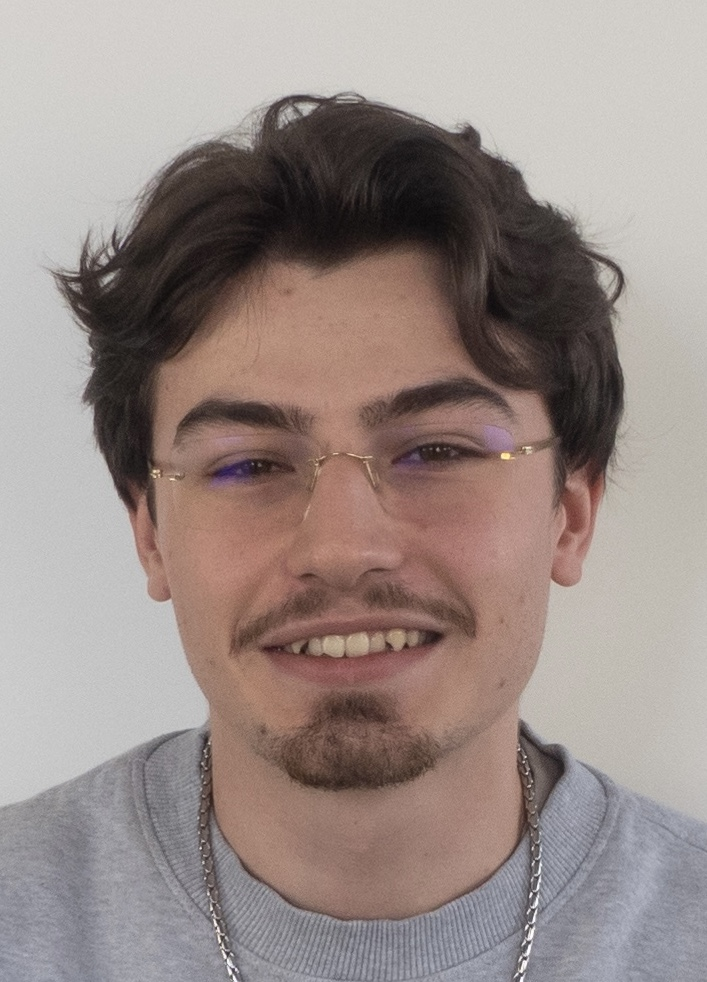
\includegraphics[width=2.5cm]{images/photo.jpg}};
            \draw [white, rounded corners=0.1cm, line width=0.1cm] 
                (current bounding box.north west) -- 
                (current bounding box.north east) --
                (current bounding box.south east) --
                (current bounding box.south west) -- cycle
                ;
        \end{tikzpicture}
        &
        % right column: name + contact
        \begin{minipage}[t]{\linewidth}
            \raggedright
            \setlength{\emergencystretch}{2em}
            \vspace*{-1.0cm}
            \textbf{\fontsize{24pt}{24pt}\selectfont Antoine Duteyrat}

            \vspace*{0.5cm}

            \normalsize
            \mbox{{\color{black}\footnotesize\faMapMarker*}\hspace*{0.13cm}Saint-Étienne}%
            \kern 0.25 cm%
            \AND%
            \kern 0.25 cm%
            \mbox{\hrefWithoutArrow{mailto:aduteyrat@gmail.com}{\color{black}{\footnotesize\faEnvelope[regular]}\hspace*{0.13cm}aduteyrat@gmail.com}}%
            \kern 0.25 cm%
            \AND%
            \kern 0.25 cm%
            \mbox{\hrefWithoutArrow{tel:+33-06-30-33-98-18}{\color{black}{\footnotesize\faPhone*}\hspace*{0.13cm}06 30 33 98 18}}%
            \kern 0.25 cm%
            \AND%
            \kern 0.25 cm%
            \mbox{\hrefWithoutArrow{https://antoinedenovembre.com/}{\color{black}{\footnotesize\faLink}\hspace*{0.13cm}antoinedenovembre.com}}%
            \kern 0.25 cm%
            \AND%
            \kern 0.25 cm%
            \mbox{\hrefWithoutArrow{https://linkedin.com/in/antoine-duteyrat/}{\color{black}{\footnotesize\faLinkedinIn}\hspace*{0.13cm}LinkedIn}}%
            \kern 0.25 cm%
            \AND%
            \kern 0.25 cm%
            \mbox{\hrefWithoutArrow{https://github.com/antoinedenovembre}{\color{black}{\footnotesize\faGithub}\hspace*{0.13cm}antoinedenovembre}}%
        \end{minipage}
    \end{tabular}
    \end{header}

% ======================================================================
% ============================= EDUCATION ==============================
% ======================================================================
    
    \section{Education}
       \begin{twocolentry}{
            \textbf{Saint-Étienne, France}\\
            \textit{Sept 2022 – Now}
            }{
            \textbf{Télécom Saint-Étienne}\\
            \textit{Master’s degree in Image Processing and Photonics}%
            }
        \end{twocolentry}


        \begin{onecolentry}
            \begin{highlights}
                \item \textbf{Relevant coursework:} Computer Vision, Machine Learning, Deep Learning, Image Processing
                \item \textbf{Relevant information:} Apprenticeship with Safety Tech in Brignais, France
            \end{highlights}
        \end{onecolentry}

		\begin{twocolentry}{
			\textbf{Chicoutimi, Canada} \\
			\textit{Jan 2022 – May 2022}
            }{
            \textbf{Université du Québec à Chicoutimi} \\
            \textit{Exchange semester in Computer Science}
            }
        \end{twocolentry}

        \begin{onecolentry}
            \begin{highlights}
                \item \textbf{Relevant coursework:} Calculus II, Android development, Data Mining
            \end{highlights}
        \end{onecolentry}

		\begin{twocolentry}{
			\textbf{Clermont-Ferrand, France} \\
			\textit{Sept 2020 – July 2022}
            }{
            \textbf{Université Clermont Auvergne} \\
            \textit{Associate's degree in Computer Science}
            }
        \end{twocolentry}

        \begin{onecolentry}
            \begin{highlights}
                \item \textbf{Relevant coursework:} OOP, Computer Networking, AI Modelling, Database management
            \end{highlights}
        \end{onecolentry}

% ======================================================================
% ============================= EXPERIENCE =============================
% ======================================================================

    \section{Experience}
        \begin{twocolentry}{
			\textbf{Brignais, France} \\
			\textit{Sept 2022 – Now}
            }{
            \textbf{Safety Tech} \\
            \textit{Image processing and engineering apprentice}
            }
        \end{twocolentry}

        \begin{onecolentry}
            \begin{highlights}
                \item Used \textbf{AGILE Scrum} methodology for embedded software development
				\item Worked with embedded systems through serial and ssh, flashing and cross-compiling embedded software via \textbf{Docker} and \textbf{CMake}
				\item Integrated classical image processing and an AI model to track the end of a truck trailer in real-time using \textbf{Cuda} and \textbf{OpenCV}
            \end{highlights}
        \end{onecolentry}

        \begin{twocolentry}{
			\textbf{Gjøvik, Norway} \\
			\textit{Aug 2024 – Oct 2024}
            }{
			\textbf{NTNU Gjøvik} \\
			\textit{Image processing for detection and tracking intern}
            }
        \end{twocolentry}

        \begin{onecolentry}
            \begin{highlights}
                \item Trained and evaluated \textbf{EfficientDet} and \textbf{YOLOv8} for animal detection in pens via \textbf{Ultralytics} and \textbf{TensorFlow}
                \item Implemented a \textbf{Barlow Twins} optimization algorithm for self-supervised learning on the EfficientDet model
            \end{highlights}
        \end{onecolentry}

% ======================================================================
% =============================== SKILLS ===============================
% ======================================================================
	
    \section{Skills and Technologies}
        \begin{onecolentry}
            \textbf{Languages:} French (native), English (C1, TOEIC 990/990) 
        \end{onecolentry}

        \begin{onecolentry}
            \textbf{Technical Skills:} C, C++, Computer Networking, Machine and Deep Learning in Python (Ultralytics, TensorFlow), Web programming, Image processing, SCRUM project management
        \end{onecolentry}

        \begin{onecolentry}
            \textbf{Interests:} Technology Trends, Teamwork, Discovering new topics and participating in innovative projects
        \end{onecolentry}

\end{document}